\documentclass[a4paper, 12pt, oneside]{article}

% Imports
\usepackage[utf8]{inputenc}  % Proper UTF-8 encoding
\usepackage[T1]{fontenc}  % More french stuff
\usepackage[francais]{babel}  % Use french language
\usepackage{csquotes}

\usepackage{graphicx}  % Images
\usepackage[top=2.5cm, bottom=2cm, left=2cm, right=2cm]{geometry}  % Margins
\usepackage{subcaption}  % Side-by-side figures
\usepackage{float}
\usepackage{wrapfig}
\usepackage{adjustbox}  % Ensmaller big things
% \usepackage{newfloat}  % Custom figure environment
% \usepackage[export]{adjustbox}

\usepackage{parskip}  % No paragraph indents

\usepackage{booktabs}  % Nice tables
\usepackage{tabulary}

\usepackage{amsmath}  % Maths
\usepackage{amsthm}  % Even more maths
\usepackage{amssymb}  % U N L I M I T E D   M A T H S
\usepackage{siunitx}  % Units
\DeclareSIUnit\bar{bar}
\usepackage[version=4]{mhchem}  % Let him cook

\usepackage[backend=biber, autolang=other, style=numeric, sorting=none]{biblatex}  % Citing
\usepackage{appendix}  % Fancy appendix

\usepackage[colorlinks,bookmarks=false,linkcolor=black,urlcolor=blue,citecolor=black]{hyperref}  % Hyperlinks
\usepackage{url}  % For bibliography urls
\usepackage{python}

\DeclareLanguageMapping{francais}{english}
\addbibresource{bibliography/bibliography.bib}


\begin{document}

\title{Rapport de Laboratoire\\Groupe N$^\circ$9\\Expérience K14: Technique du vide et Point triple de l’azote}
\author{Martin \textsc{Godet} \and Tom \textsc{Vadot}}
\date{\today}

\maketitle

% \begin{figure}[h]
%     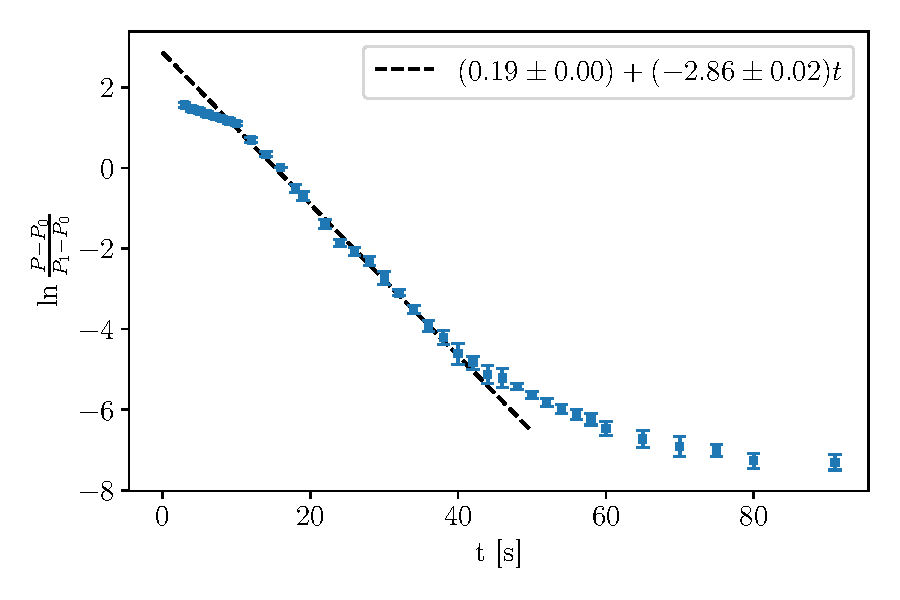
\includegraphics{figures/cinetique_palettes.pdf}
% \end{figure}

\section{Introduction}

Dans le contexte de la crise climatique et énergetique, les moyens de chauffage restent une question majeure. En 2022, 56.8\% des habitations en Suisse étaient chauffées aux énergies fossiles, dont 39.3\% au mazout et 17.5\% au gaz \cite{chauffage}. Ces méthodes de chauffage fonctionnent sur le principe de combustion de liquide ou gaz afin de produire de la chaleur, permettant de réchauffer de l'eau, qui circule dans le circuit de chauffage par exemple. En plus de l'isolation des batiments, la qualité et la densité énergétique du combustible sont clés pour limiter l'impact du chauffage sur le climat. Il est estimé qu'environ 25\% de l'énergie produite dans le monde est utilisée pour réchauffer et refroidir les habitations et espaces commerciaux \cite{energie-chauffage}. Un enjeu essentiel est donc de connaître l'efficacité des différents combustibles.

Lors de cette expérience, le pouvoir calorifique ainsi que les émissions en \ce{CO2} de deux combustibles liquides: un gaz de camping composé à 80\% de butane et 20\% de propane, et un mélange éthanol-méthanol à 88\%-12\%, seront déterminés. De plus, la valeur théorique de ces combustibles sera calculée et comparée à la valeur expérimentale obtenue afin d'étudier la fiabilité du montage utilisé.
\section{Théorie}






\paragraph*{Cycle de Stirling en pompe à chaleur}
Un moteur de Stirling peut également fonctionner en mode pompe à chaleur ou machine frigorifique, la seule différence étant l'intérêt dans l'apport ou l'extraction de chaleur. Il s'agit dans ce cas d'entraîner le cycle à l'aide d'un moteur extérieur. Selon le sens de rotation de l'arbre les flux de chaleurs produits par la pompe à chaleur seront dans des sens différents, dans le même sens pour une même rotation et dans le sens inverse dans le cas contraire. TODO: dire que équation est la même à un signe près

Les valeurs du rendement se basent sur le même concept mais les flux d'énergies considérés ne sont plus les même. Dans le cas d'un cycle frigorifique, la puissance fournie est la puissance du moteur d'entraînement \(P_{moteur}\) et la grandeur d'intérêt est le flux de chaleur évacué \(\phi\). Le rendement est donc donné par l'équation:
\begin{equation}
    \rho = \frac{\phi}{\P_{moteur}}
    \label{eq:rend-frigo}
\end{equation}
\section{Demarche Expérimentale}


\begin{minipage}{\textwidth}
    \begin{wrapfigure}{R}{0.5\textwidth}
        \centering
        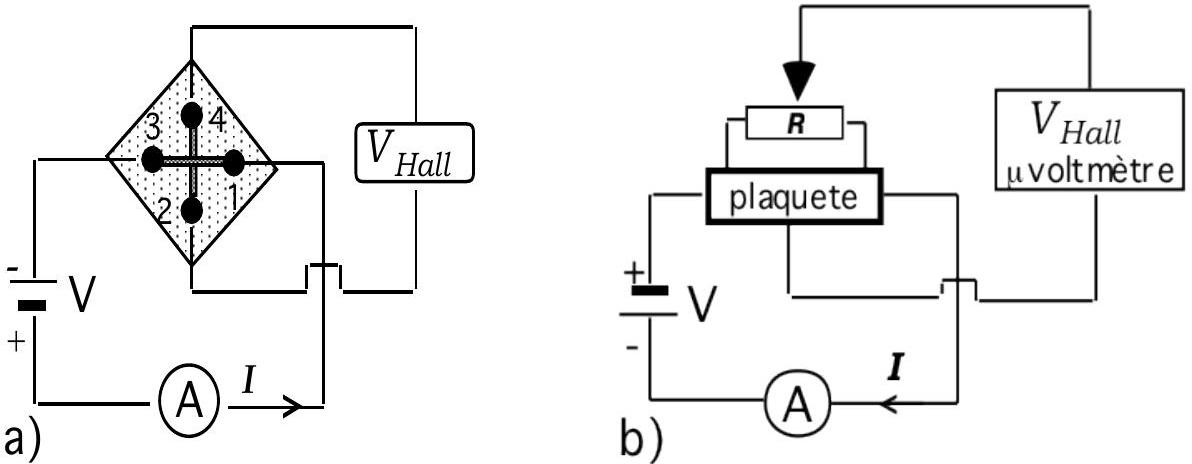
\includegraphics[width=\linewidth]{figures/montage.png}
        \caption{Dispositif expérimental utilisé pour constater l'effet Hall \cite{notice}}
        \label{fig:montage}
        \vspace*{1cm}
    \end{wrapfigure}

    Le montage expérimental \autoref{fig:montage} utilisé dans cette expérience est composé de deux bobines en cuivre dans lequel un générateur permet de faire passer un courant continu créant ainsi un champ magnétique dans l'entrefer. Un échantillon peut être placé au niveau de celui-ci et ainsi permet de mesurer une tension de Hall quand un courant le traverse. Deux multimètre sont utilisés pour mesurer le courant entrant dans l'échantillon et pour mesurer la tension de Hall. La résistance interne du multimètre pris comme microvoltmètre est supposée suffisament grande pour ne pas affecter les mesures.
\end{minipage}

Les mesures du champ magnétique seront elles effectuées à l'aide d'un teslamètre qu'il convient de mettre à zéro avant le début des mesures. Il est important de ne pas trop faire bouger la tête de mesure durant son utilisation car l'intensité du champ magnétique mesurée dépend fortement de la position et de l'orientation.

\begin{minipage}{\textwidth}
    \begin{wrapfigure}{R}{0.5\textwidth}
        \centering
        \begin{subfigure}{0.25\textwidth}
            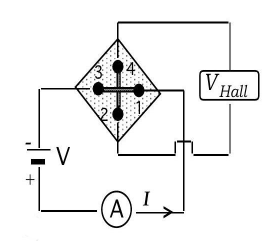
\includegraphics[width=\linewidth]{figures/circuit_4branch.png}
            \caption{}
            \label{fig:4branch}
        \end{subfigure}%
        \begin{subfigure}{0.25\textwidth}
            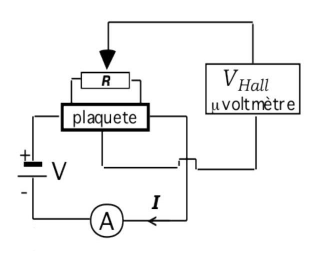
\includegraphics[width=\linewidth]{figures/circuit_5branch.png}
            \caption{}
            \label{fig:5branch}
        \end{subfigure}
        \caption{Méthodes de mesure de la tension de Hall à 4 contacts (a) et à 5 contacts (b) \cite{notice}}
        \label{fig:circuit}
        \vspace*{1cm}
    \end{wrapfigure}

    Afin de mesurer la tension de Hall deux types de branchements sont possibles. Le premier à 4 contacts \autoref{fig:4branch} permet de prendre plusieurs mesures aisément mais est affecté par une tension résiudelle présente même avec un champ magnétique nul. Le deuxième à 5 contacts \autoref{fig:5branch} dispose d'un potentiomètre branché en parallèle afin de se débarasser de cette tension résiduelle. 
    
    Les mesures à 4 contacts ont été faites sur deux échantillons d'InP dopés au Si d'épaisseurs 1 \si{\micro\meter} et 2 \si{\micro\meter}. Les mesures à 5 contacts ont été faites sur un échantillon d'argent Ag d'épaisseur 1.9 \si{\micro \meter}, un de cuivre Cu d'épaisseur 1.6 \si{\micro \meter} et un de bismuth Bi d'épaisseur 3 \si{\milli \meter}.

    La détermination des valeurs de \(R_H\) et \(N\) peut se faire par la mesure de \(V_H\) en fonction de \(I\) ou de \(V_H\) en fonction de \(B\). Ces deux ensembles de mesures ont été effectués pour chaque échantillon.
    
    De plus l'hystérèse de la génération du champ magnétique par les bobines sera observé en parcourant une gamme d'intensité allabt de -6 à 6 \si{\ampere} en diminuant puis en augmentant le courant afin de relever le champ magnétique \(B\) correspondant.
    
\end{minipage}
\section{Résultats}

\paragraph*{Mesures}
L'approche critique a été réalisée en commencant à \(h_0 = 920.0 \pm 0.1\) mm. À chaque hauteur, le courant \(I\), ainsi que le nombre de neutrons \(n\) et temps \(t\) écoulé ont été mesurés. Le taux taux de compte \(C\) est alors déterminé avec \(C = n/t\). Les hauteurs où les mesures ont été réalisées ainsi que les valeurs mesurées sont reportées dans le \autoref{tab:mesures}.

\begin{table}[h]
    \centering
    \begin{tabular}{ |c||c|c|c|c|c| }
        \hline
        h [mm] & I [nA] & n & t [s] & C [\si{\per\second}] \\
        \hline\hline
        \(920.0 \pm 0.1\) & \(0.30 \pm 0.02\) & \(10006 \pm 100\) & \(391.6 \pm 0.1\) & \(25.5 \pm 0.3\) \\
        \(930.0 \pm 0.1\) & \(0.42 \pm 0.02\) & \(10010 \pm 100\) & \(279.8 \pm 0.1\) & \(35.7 \pm 0.4\) \\
        \(938.3 \pm 0.1\) & \(0.67 \pm 0.02\) & \(10002 \pm 100\) & \(188.2 \pm 0.1\) & \(53.1 \pm 0.5\) \\
        \(943.1 \pm 0.1\) & \(1.1 \pm 0.2\) & \(10015 \pm 100\) & \(126.9 \pm 0.1\) & \(78.9 \pm 0.8\) \\
        \hline
    \end{tabular}
    \caption{Hauteur d'eau dans le réacteur, courant, compte, temps de compte et taux de compte obtenus}
    \label{tab:mesures}
\end{table}

\paragraph{Estimations avec courant}
En accord avec la théorie, la hauteur critique est proportionnelle à l'inverse du courant. En utilisant la méthode décrite dans la démarche expérimentale, la hauteur critique \(h_c\) a été déterminée. Une estimation sur l'erreur est obtenue de manière graphique, comme décrit dans \autoref{sec:erreurs}. Les résultats sont présentés dans \autoref{fig:hc_intensite}. Une hauteur critique entre 950 et 955 a alors été trouvé. Expérimentalement, l'opérateur a montré que la hauteur critique était \(h_c = 952.2 \pm 0.1\) mm.

\begin{figure}[H]
    \centering
    \begin{subfigure}{0.48\linewidth}
        \centering
        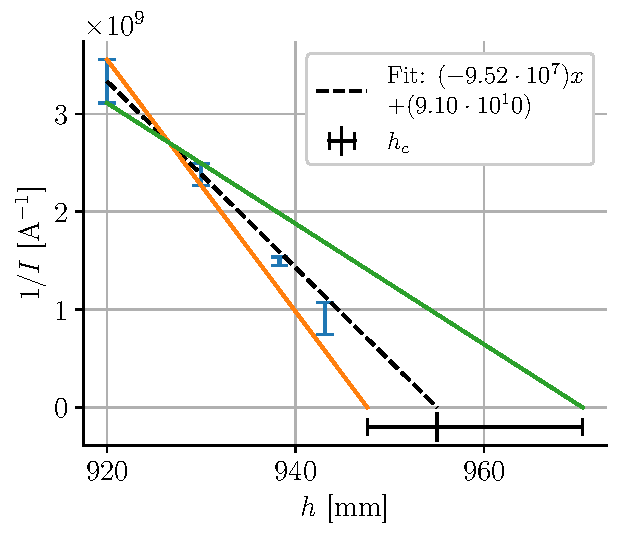
\includegraphics[width=\linewidth]{figures/h_I_pair12.pdf}
        \caption{}
        \label{fig:hc_I_12}
    \end{subfigure}
    \begin{subfigure}{0.48\linewidth}
        \centering
        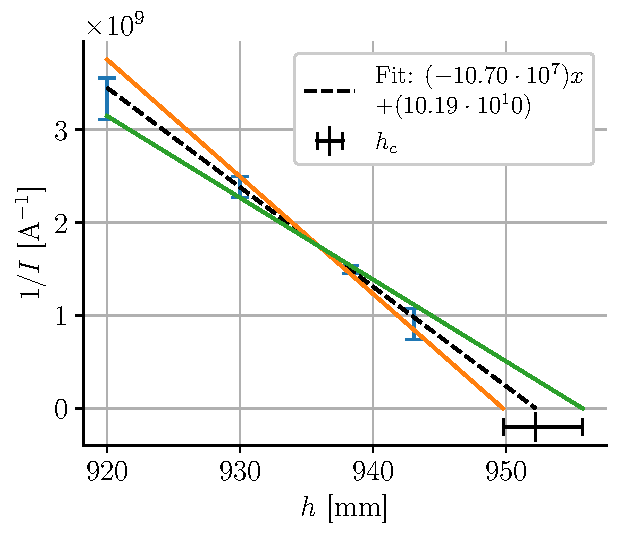
\includegraphics[width=\linewidth]{figures/h_I_pair23.pdf}
        \caption{}
        \label{fig:hc_I_23}
    \end{subfigure}
    \begin{subfigure}{0.48\linewidth}
        \centering
        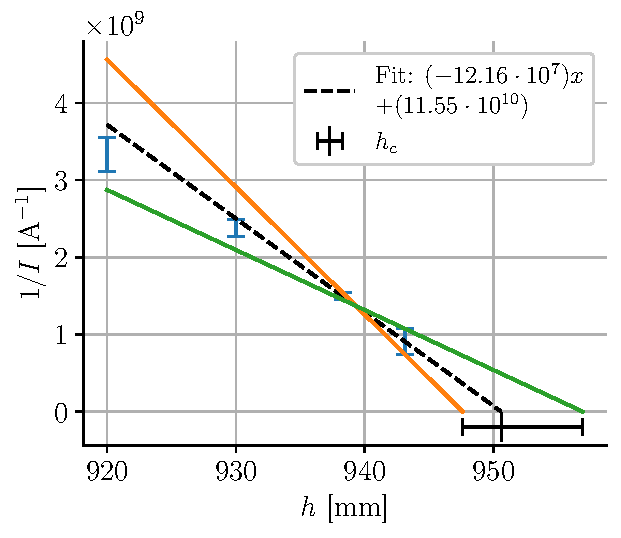
\includegraphics[width=\linewidth]{figures/h_I_pair34.pdf}
        \caption{}
        \label{fig:hc_I_34}
    \end{subfigure}
    \begin{subfigure}{0.48\linewidth}
        \centering
        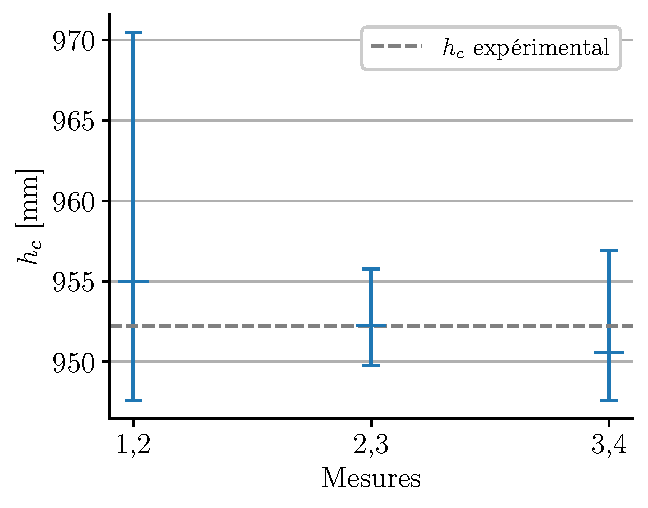
\includegraphics[width=\linewidth]{figures/hc_results_I.pdf}
        \caption{}
        \label{fig:hc_I}
    \end{subfigure}
    \caption{Estimations de \(h_c\) avec une régression linéaire en utilisant les mesures (a) 1 et 2, (b) 2 et 3, (c) 3 et 4. En (d) les hauteurs critiques \(h_c\) trouvées, ainsi que l'estimation de l'erreur sur la valeur trouvée.}
    \label{fig:hc_intensite}
\end{figure}

\paragraph*{Estimations avec taux de compte}
feur
\section{Discussion}


\paragraph*{Types de magnétisation}
Plusieurs types de magnétisation des matériaux ont été trouvés au cours de cette expérience. Tout d'abord les deux matériaux contenant de l'acier ont été déterminés comme fortement ferromagnétiques avec de hautes valeurs pour \(mu_r\) dans le transformateur cylindre. Il est donc possible de déduire que l'acier en général est un alliage avec un caractère ferromagnétique et une très bonne perméabilité au magnétisme. Les caractéristiques 
\section{Conclusion}

Lors de cette expérience la relaxation anélastique de plusieurs échantillons de matériaux différents a été étudié, sous plusieurs conditions de température notamment. Ainsi leur module de Young \(E\) et leur capacité d'amortissement \(Q^{-1}\) ont été calculés. Cela donne des informations importantes sur le comportement sous la contrainte de ces matériaux. Entre les trois échantillons testés, l'acier doux avait la plus grande capacité d'amortissement. Ce résultat est donc cohérent avec l'utilisation de l'acier dans la construction comme matériaux principal pour la résistance parasysmique \cite{acier-construction}. Les méthodes utilisées ici permettent également d'obtenir des informations sur la structure microscopique des matériaux. La concentration en défauts interstitiels indique la pureté du cristal et comparer plusieurs échantillons du même matériau avec l'expérience présentée ici pourra permettre d'évaluer leurs puretés respectives.


% Bibliography
\nocite{*}  % While writing report, ignore unused citations
\printbibliography

\newpage

\begin{appendices}
\section{Calcul d'erreurs}
\label{sec:erreurs}

Les erreurs sur les mesures sont données dans le \autoref{tab:erreurs}.

\begin{table}[h]
    \centering
    \begin{tabulary}{\textwidth}{C C}
        \toprule
        Variable & Erreur \\
        \midrule
        Frequence \(\omega\) [\si{\radian\per\second}] & est \\
        \bottomrule
    \end{tabulary}
    \caption{Erreurs estimées sur les mesures}
    \label{tab:erreurs}
\end{table}

\paragraph*{Regression linéaire}
Les erreurs sur les régressions linéaires \(y = ax + b\) sur les mesures \((x_i, y_i) ; i = \{1, \dots, n\}\) sont donnés par \cite{erreursmesure}:

\begin{equation}
    \label{eq:erreur:fit}
    \begin{aligned}
        (\Delta a)^2 &= \frac{\sum_{i=1}^{n}(y_i - (a x_i + b))^2}{(n-2) \sum_{i=1}^{n}(x_i - \bar{x})^2}\\
        \Delta b &= \bar{x} \Delta a + a \Delta \bar{x}
    \end{aligned}
\end{equation}

En pratique, ces valeurs sont calculées par la bibliothèque python \texttt{numpy}.

\paragraph*{Formules d'erreurs}

Erreur sur feur:
\begin{equation}
    feur
\end{equation}

Toutes ces erreurs sont calculées en pratique par la bibliothèque \texttt{uncertainties}.

\end{appendices}

\end{document}
